\documentclass[twocolumns]{IEEEtran}
\usepackage[utf8]{inputenc}
\usepackage[english]{babel}

\usepackage{tikz}
\usepackage{graphicx}

\usepackage{bm}
\usepackage{amsmath}
\usepackage{mathtools}

\usepackage{authblk}
\usepackage{hyperref}
\usepackage{blindtext}

\usetikzlibrary{fit,positioning,arrows,automata,calc}

\setlength{\parindent}{0pt}%

% document meta data
\title{Project Report:\\ Part-Of-Speech Tagging and Named Entity Recognition with Probabilistic Graphical Models}
\author[1]{Clemens Biehl (clemens.biehl@stud.tu-darmstadt.de)}
\author[1]{Daniel Wehner (daniel.wehner@stud.tu-darmstadt.de)}
\author[1]{Fabian Otto (fabian.otto@stud.tu-darmstadt.de)}
\affil[1]{Technische Universität Darmstadt}

\DeclareMathOperator*{\argmax}{arg\,max}
\DeclareMathOperator*{\argmin}{arg\,min}
\newcommand{\indep}{\rotatebox[origin=c]{90}{$\models$}}

\tikzset{
  main/.style={circle, minimum size = 5mm, thick, draw =black!80, node distance = 10mm},
  connect/.style={-latex, thick},
  box/.style={rectangle, draw=black!100}
}

\begin{document}
\maketitle
\begin{abstract}
Natural language processing is an increasingly important task, in which Part-of-Speech (POS) tagging and Named Entity Recognition (NER) are important steps for complex semantic processing tasks. Therefore, in this project we evaluate different probabilistic graphical models -- Na\"ive Bayes, Hidden Markov Models and Conditional Random Fields -- for those two tasks and additionally compared the performance of different handcrafted features as well as GloVe word embeddings. Furthermore, we also evaluated the models using a significantly reduced size of the training data set. The results indicate that the CRF model performs best in various settings almost irrespective of the features chosen. For POS tagging HMMS and CRFs tend to work better since they operate on sentence-level. 
\end{abstract}

\section{Introduction}
Natural Language Processing (NLP) is the application of computational techniques for the automatic analysis and representation of human language. This field becomes increasingly interesting as the number of available resources on the web is increasing and millions of websites and documents can be accessed and processed. Making use of this large amount of unstructured data to enable and improve computational natural language understanding is therefore a task worth investigating more in depth \cite{nlpintro}.

The tasks of \textbf{part-of-speech (POS) tagging} as well as \textbf{named entity recognition (NER)} are required for various downstream tasks such as \textbf{question answering} or \textbf{information extraction}. However, these tasks are non-trivial, since natural language expressions can be ambiguous in multiple ways. For instance a word can have multiple parts-of-speech and a term like \textit{Florence} might refer to either a named entity \texttt{PERSON} or \texttt{LOCATION} \cite[cf. pages 167-169]{Jurafsky}.

\textbf{The goal of this project} is to compare different approaches of manual feature engineering and word embeddings as well as different probabilistic graphical models on the tasks of part-of-speech tagging and named entity recognition. The \textbf{Groningen Meaning Bank} of University of Groningen is going to be used as a training corpus \cite{Bos2017GMB}.

\section{Literature Review}
\subsection{Natural Language Processing Pipeline}

Solving a natural language processing (NLP) problem necessitates a pipeline -- a sequence of tasks which have to be dealt with in order. POS tagging is one key part in almost every NLP pipeline. It can e.\,g. be used to facilitate the identification of named entities or constituents and dependencies. Figure \ref{fig:nlp-pipeline} depicts such an NLP pipeline.

\begin{figure}[h]
    \centering
    \fbox{\includegraphics[scale=0.3]{nlp_pipeline}}
    \caption{Natural Language Processing consists of several steps.
        These steps can be arranged in an NLP pipeline.}
    \label{fig:nlp-pipeline}
\end{figure}

As can be seen in Figure \ref{fig:nlp-pipeline} POS tagging is applied at an early stage of the pipeline which emphasizes its very importance. 
Almost all tasks in NLP rely on POS tagging making its performance crucial for the performance of the entire pipeline.

\subsection{Part-Of-Speech Tagging}
POS tagging refers to the assignment of part-of-speech tags to words in a text, i.\,e. the task is to decide whether a word is a noun (\texttt{NN}), plural-noun (\texttt{NNS}), verb (\texttt{VB*}), etc. There are several \textit{rule-based} and \textit{stochastic algorithms} to perform this classification of word categories.

While most words in large text corpora are nouns, accurate part-of-speech tagging is still a challenging task, because words can be ambiguous (polysemy), i.\,e. can have different parts-of-speech. One way to distinguish between the different possible parts-of-speech for a particular word occurrence is to incorporate the context of this word, i.\,e. the surrounding tokens, as well as morphological features such as affixes, prefixes, etc. \cite[cf. pages 167-170]{Jurafsky}

State-of-the-art POS taggers reach a word-level accuracy of 0.97 to 0.98, whereas the sentence-level performance is around 0.56 \cite{postaggingbenchmark} \cite{manningpostagging} \cite{dlnerbenchmark}.

\vspace*{3mm}
\textbf{Example:}

\begin{quote}
    [\textbf{She} | \texttt{PRP}] [\textbf{sells} | \texttt{VBZ}] [\textbf{seashells} | \texttt{NNS}] [\textbf{on} | \texttt{IN}] [\textbf{the} | \texttt{DT}] [\textbf{seashore} | \texttt{NN}] [\textbf{.} | \texttt{.}]
\end{quote}

\subsection{Named Entity Recognition}
Named Entity Recognition (NER) is the task of identifying spans of text that represent proper names and classifying these as a particular type of entity such as \texttt{PERSON}, \texttt{LOCATION} or \texttt{DATE}, etc. (see example below)
A model which seeks to solve this task needs to deal with ambiguities arising from the fact that some words (e.\,g. \textit{Florence}) could refer to multiple entities (e.\,g. \texttt{PERSON}, \texttt{LOCATION}).

Again, the context of a named entity can be a useful feature for NER and help to disambiguate between multiple entity types in such cases \cite[cf. pages 761-765]{Jurafsky}. Deep learning based methods for NER achieve an F1 measure of about 0.91 on the CoNLL-2003 test set\cite{dlnerbenchmark}.

\vspace*{3mm}
\textbf{Example:}

\begin{quote}
\textit{The decision by the independent member of parliament \colorbox{blue!30}{Andrew Wilkie} to withdraw his support for the minority \colorbox{red!30}{Labor} government sounded dramatic but it should not further threaten its stability. When, after the \colorbox{yellow!30}{2010} election, \colorbox{blue!30}{Wilkie}, \colorbox{blue!30}{Rob Oakeshott}, \colorbox{blue!30}{Tony Windsor} and the \colorbox{red!30}{Greens} agreed to support \colorbox{red!30}{Labor}, they gave just two guarantees: confidence and supply.}
\end{quote}

\vspace*{2mm}
Colours: \colorbox{blue!30}{\texttt{Person}} -- \colorbox{red!30}{\texttt{Organization}} -- \colorbox{yellow!30}{\texttt{Date}}

\subsection{Na\"ive Bayes}
The Na\"ive Bayes classifier is a generative model which assumes that all subsets of features are independent given the class label: $(\bm{X} \indep \bm{Y} \vert C)$ Thus, the maximum aposteriori (MAP) can be computed as follows:

\begin{equation*}
    C_{MAP}^* = \argmax_{C \in \mathcal{C}} P(C) \cdot \prod_{i=1}^m P(x_i \vert C)
\end{equation*}

\begin{figure}[h]
	\centering
	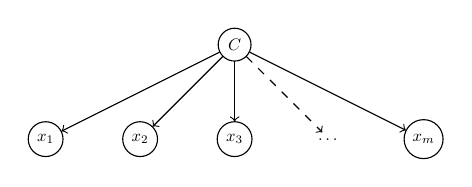
\begin{tikzpicture}[
		scale=0.6,
		every node/.style={scale=0.6}
	]

		\node[circle,draw=black] (C) at (0,2) {$C$};
		\node[circle,draw=black] (X1) at (-4,0) {$x_1$};
		\node[circle,draw=black] (X2) at (-2,0) {$x_2$};
		\node[circle,draw=black] (X3) at (0,0) {$x_3$};
		\node (Xi) at (2,0) {$\dots$};
		\node[circle,draw=black] (Xm) at (4,0) {$x_m$};
		\draw[->] (C) -- (X1);
		\draw[->] (C) -- (X2);
		\draw[->] (C) -- (X3);
		\draw[->,dashed] (C) -- (Xi);
		\draw[->] (C) -- (Xm);
	\end{tikzpicture}
	\caption{Na\"ive Bayes as a probabilistic graphical model. The features $\bm{x}$ are independent given the class label $C$.}
\end{figure}

Na\"ive Bayes operates on token level, i.\,e. the context cannot be incorporated into the predictions. In the context of our experiments the Na\"ive Bayes classifier is going to serve as a baseline for the performance in both tasks POS tagging and NER. The implementation of the \textit{nltk} framework is going to be used.\footnote{\texttt{\url{https://www.nltk.org/}}}

\subsection{Hidden Markov Models}
Hidden Markov models (HMMs) are directed probabilistic graphical models which -- in contrast to the Na\"ive Bayes algorithm (which classifies on token level) -- operate on sequence level, i.\,e. they assign the most probable sequence of labels. This allows it to incorporate the context into the prediction. The latter property is especially useful for natural language processing, where words can have different meanings depending on the context (words around the word of interest.) In POS tagging we want to find the best tag sequence $\bm{t}^*$ given an input sequence of words $\bm{w}$:

\begin{equation*}
    \bm{t}^* = \argmax_{\bm{t}} P(\bm{t} \vert \bm{w})
        \propto \argmax_{\bm{t}} P(\bm{w} \vert \bm{t})P(\bm{t})
\end{equation*}

Unfortunately, this equation is hard to compute. This is why HMMs make two simplifying assumptions which facilitate the computation process:

\begin{enumerate}
    \item The probability of a word appearing depends only on its own POS tag
        (it is independent of all the other words and tags around it):
        $P(\bm{w}\vert\bm{t}) = \prod_{i=1}^n P(w_i \vert t_i)$
    \item Due to the sparsity of the training data it is in general hard to estimate
        $P(\bm{t})$ well enough. Hence the so-called \textbf{Markov property} is assumed, i.\,e. the probability of a particular state depends solely on the previous state and not on earlier ones.\footnote{\textit{The future is independent of the past given the present}} \cite[cf. pages 211-212]{Jurafsky}:
        $P(w_i|w_1,\dots,w_{i-1}) = P(w_i|w_{i-1})$
\end{enumerate}

\begin{figure}[h]
    \centering
    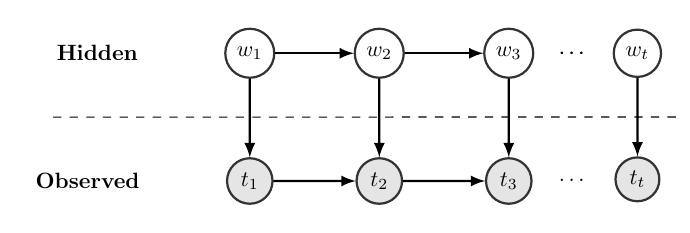
\begin{tikzpicture}[scale=0.1, every node/.style={scale=0.8}]
      \node[box,draw=white!100] (Latent) {\textbf{Hidden}};
      \node[main] (L1) [right=of Latent] {$w_1$};
      \node[main] (L2) [right=of L1] {$w_2$};
      \node[main] (L3) [right=of L2] {$w_3$};
      \node[main] (Lt) [right=of L3] {$w_t$};
      \node[main,fill=black!10] (O1) [below=of L1] {$t_1$};
      \node[main,fill=black!10] (O2) [below=of L2] {$t_2$};
      \node[main,fill=black!10] (O3) [below=of L3] {$t_3$};
      \node[main,fill=black!10] (Ot) [below=of Lt] {$t_t$};
      \node[box,draw=white!100,left=of O1] (Observed) {\textbf{Observed}};
      \path (L3) -- node[auto=false]{\ldots} (Lt);
      \path (L1) edge [connect] (L2)
            (L2) edge [connect] (L3)
            (L3) -- node[auto=false]{\ldots} (Lt);
      \path (O1) edge [connect] (O2)
            (O2) edge [connect] (O3)
            (O3) -- node[auto=false]{\ldots} (Ot);
      \path (L1) edge [connect] (O1);
      \path (L2) edge [connect] (O2);
      \path (L3) edge [connect] (O3);
      \path (Lt) edge [connect] (Ot);
    
      % draw the dashed line
      \draw [dashed, shorten >=-0.5cm, shorten <=-0.5cm]
          ($(Latent)!0.5!(Observed)$) coordinate (a) -- ($(Lt)!(a)!(Ot)$);
    \end{tikzpicture}
    \caption{An example of a Hidden Markov model.}
    \label{fig:hmm}
\end{figure}

Putting all components together the HMM model can be written as:

\begin{equation*}
    \bm{t}^* = \argmax_{\bm{t}} \prod_{i=1}^n P(w_i \vert t_i)
        \cdot P(t_i \vert t_{i-1})
\end{equation*}

In the task of POS tagging the probabilities can be obtained by counting the occurrences in a large training corpus (e.\,g. the \textsc{Brown} corpus):

\begin{align*}
    P(t_i \vert t_{i-1})    &= \frac{\#\{t_{i-1, t_i}\}}{\#\{t_{i-1}\}} \\[2mm]
    P(w_i \vert t_i)        &= \frac{\#\{t_i, w_i\}}{\#\{t_i\}}
\end{align*}

Among others the \textbf{Viterbi} algorithm (dynamic programming approach) can be used in order to compute the best matching tag sequence.

\vspace*{3mm}
\textbf{Example use cases for HMMs:} In \cite{Awasthi2006} the authors use Brant's TnT tagger \cite{Brants:2000:TSP:974147.974178} for POS tagging which uses Hidden Markov Models (HMM). Based on the error the tagger makes they additionally learn transformation rules which should correct the errors. 
The authors report an F1-Score of 79.66\,\% (without error correction) and 80.74\,\% with error correction. 

\subsection{Conditional Random Fields (CRFs)}
In general, the CRF algorithm can be viewed as logistic regression applied to sequence data and belongs to the family of discriminative machine learning approaches. Conditional Random Fields (CRF) are also closely related to hidden markov models. But unlike HMMs they are of undirected nature. \cite{Sutton:2012} When making predictions CRFs have to take the previous context into account. This is achieved by using so-called feature functions. In the context of part-of-speech tagging the feature function could be of the following type:

\begin{equation*}
    f(\bm{X}, i, l_{i-1}, l_i)
\end{equation*}

Where $\bm{X}$ is the set of input vectors, $i$ the position of the data point we want to predict and $l_{i-1}$ / $l_i$ the label of the previous word and the current word respectively. The conditional probability $P(y \vert \bm{X}, \lambda)$ can be computed as follows:

{\footnotesize
\begin{align*}
    P(\bm{y} \vert \bm{X}, \bm{\lambda})
        &=  \frac{1}{Z(\bm{X})}\exp\left\{
                \sum_{i=1}^n \sum_j \lambda_j f_i(\bm{X}, i, y_{i-1}, y_i)
            \right\} \\
    Z(\bm{X})
        &=  \sum_{y' \in \bm{Y}} \sum_{i=1}^n \sum_j \lambda_j f_j(\bm{X}, i, y'_{i-1}, y'_i) 
\end{align*}}

For the training procedure it is required that the training data be i.i.d. (independent and identically distributed): $\mathcal{D} = \left\{ (x^{(1)}, y^{(1)}, (x^{(2)}, y^{(2)}), \dots, (x^{(m)}, y^{(m)}\right\}$. The task is to find the optimal parameters $\bm{\lambda}^*$. For that, the negative log-likelihood is used:

{\scriptsize
\begin{align*}
    \mathcal{L}(\bm{\lambda}, \mathcal{D})
        &= -\log\left(
            \prod_{k=1}^m P(\bm{y}^{(k)} \vert \bm{x}^{(k)}, \bm{\lambda})
        \right) \\
        &= -\sum_{k=1}^m \log\left[
            \frac{1}{Z(\bm{x}^{(m)})}\exp\left\{
                \sum_{i=1}^n \sum_j \lambda_j f_j(\bm{x}^{(m)}, i, y_{i-1}^k, y_i^k)
            \right\}
        \right]
\end{align*}}

Optimizing the above equation yields the optimal parameter configuration $\bm{\lambda}^*$. As it turns out this optimization problem is convex and has therefore no local optima. The global maximum of the function can be found by minimizing it:

\begin{equation*}
    \bm{\lambda}^* = \argmin_{\bm{\lambda}} \left\{
        \mathcal{L}(\bm{\lambda}, \mathcal{D}) + \underbracket{
            C \frac{1}{2} \Vert \bm{\lambda} \Vert^2
        }_{\text{regularization}}
    \right\}
\end{equation*}

The parameter $C$ controls the degree of regularization which is a method to prevent overfitting. In the equation above the $L_2$ regularization is employed.

%It is a discriminative approach which models the conditional probability $p(\boldsymbol{y} \vert \boldsymbol{x})$ and refrains from modeling the marginal $p(\boldsymbol{x})$. \cite{Lafferty}  

\vspace*{3mm}
\textbf{Example use cases for conditional random fields:}
The authors of \cite{Avinesh2006} make use of a conditional random field ('CRF++, Yet another CRF package') in order to perform POS tagging for the language Hindi. The authors of the paper trained the model on 21.000 words and report an accuracy of 82.67\,\%.

Named entity recognition represents another NLP problem which can be addressed by CRFs \cite{McCallum2003}. The authors report results on the CoNLL-2003 named entity recognition shared task consisting of tagged news articles. They achieved an F1-score of 84.04\,\% (for the English language) and 68.11\,\% (for the German language). The classes were as follows: \texttt{PERSON}, \texttt{LOCATION}, \texttt{ORGANIZATION} and \texttt{MISC}.

\section{Methodology and Objective}
\subsection{General Objective}
This project seeks to accurately identify POS and NE tags by using different probabilistic graphical models. 
Further, this project utilizes two distinct feature sets -- manually engineered features (1) and GloVe word embeddings (2) \cite{pennington} -- in combination with a Na\"ive Bayes and a CRF. 
Additionally a hidden Markov model is evaluated given the token sequence as input.

For computing the Na\"ive Bayes model, the \textit{nltk} framework\footnote{\texttt{\url{https://www.nltk.org/}}} is going to be used, the hidden Markov model is based on the implementation from nltk\footnote{\texttt{\url{https://www.nltk.org/_modules/nltk/tag/hmm.html}}} as well, since it already provides an interface for conveniently processing natural language. The \textit{python-crfsuite}\footnote{\texttt{\url{https://python-crfsuite.readthedocs.io/en/latest/}}} package provides a wrapper to \textit{CRFSuite} as an implementation of linear chain conditional random fields which is used in this project.

All approaches are evaluated with the micro-averaged F1 measure as harmonic mean between Precision and Recall and compared to up-to-date benchmarks.

% andrew2007scalable

\subsection{Research questions}
\begin{enumerate}
\item[\textbf{Q1}] How do CRF and HMM compare to the baseline of Na\"ive Bayes? 
\item[\textbf{Q2}] Which handcrafted features are suited best for the different models in order to reach a high accuracy for POS tagging and NER?
\item[\textbf{Q3}] How do handcrafted features compare to word embeddings?
\item[\textbf{Q4}] Can graphical models with well-engineered features beat deep learning benchmarks?
\end{enumerate}

\section{Results and Evaluation}

For our evaluation we assessed different feature combinations. These included:

\vspace*{2mm}
\begin{itemize}
    \item word features:
    \begin{itemize}
        \item \textbf{w:} the word itself
        \item \textbf{l:} the lowercased word
        \item \textbf{s:} the stem of the word
    \end{itemize}
    \item unknown word features (\textbf{uwf}):
    \begin{itemize}
        \item word shapes\footnote{The term \textit{word shape} refers to an abstract representation of a character sequence in which alphanumerical characters are replaced by \textit{x} or capital \textit{X} and digits are replaced by \textit{d}} (e.\,g. Hello $\longrightarrow$ Xxxxx)
        \item capitalization
        \item affixes
    \end{itemize}
    \item bigram features (\textbf{bf})
    \item a combination of all of the above
\end{itemize}
\vspace*{2mm}

For named entity recognition we also included the gold POS tags (of the current token in a sequence as well as the previous token) into our feature set (\textbf{pos}).

All results are evaluated on word-level using the micro averaged F1 score and by sentence-level accuracy.

%TODO: Describe training procedure in more detail
All models are trained using a \textbf{maximum likelihood estimation} approach. For the Na\"ive Bayes model the number of feature occurrences per label is counted, the sufficient statistics for the HMM model are obtained by collecting the frequencies of transitions between hidden states and token observations within each state.
The CRF model is trained using the \textbf{orthant-wise limited-memory quasi-Newton} optimization algorithm, a variant of the L-BFGS optimization algorithm, which optimizes the $L_1$-regularized log-likelihood \cite{owlqn}. Using L-BFGS optimization without $L_1$ regularization led to a notable decrease of 0.017 in sentence-level accuracy for the best CRF model for NER.

\subsection{Part-of-Speech Tagging}
Compared to the Bi-LSTM baseline used by the creators of the data set, Bjerva et al. \cite{bjervabaseline}, we found that our CRF model achieves a higher F1 score. However, the authors used an older version of the Groningen Meaning Bank comprising less data. Further, we did not find any additional work utilizing the Groningen Meaning Bank to compare our results with.

\vspace*{3mm}
% Naive Bayes
\colorbox{gray!30}{\textbf{Na\"ive Bayes}}

Table \ref{nbpos} shows the results of a Na\"ive Bayes classifier using only the word features. This setting already achieves an F1 score of approximately 0.92. This can be explained by the unbalanced data set which mainly contains nouns (\texttt{NN}). Adding bigram features significantly increased the F1 score performance to 0.957 and almost doubled the sentence-level accuracy. In general we found that Na\"ive Bayes performs poorly on sentence-level accuracy. This is due to the word level classification which also explains the increase by using bigram features. In contrast, the unknown word features led to a decrease in performance. By analyzing the probabilities and features importance we did not find any clear evidence for the performance decrease caused by the unknown word features.

\begin{table}[h]
    \centering
    \caption{POS Performance Evaluation of Na\"ive Bayes}\label{nbpos}
	\scalebox{1.1}{
	\begin{tabular}{| c | c | c |}
		\hline
		\multicolumn{3}{| c |}{\textbf{Na\"{i}ve Bayes} [POS]}
		\\ \hline\hline
		\textbf{Features}		&	\textbf{F1 score}		& 	\textbf{Acc (word / sent)}
		\\ \hline\hline
		w, l, s 				& 	0.927				& 	0.927 / 0.240
		\\ \hline
		w, l, s, uwf				&	0.928				&	0.928 / 0.241
		\\ \hline
		w, l, s, bf 				& 	0.957 				&	0.957 / 0.467
		\\ \hline
		w, l, s, uwf, bf			& 	0.949 				& 	0.949 / 0.369
		\\ \hline
	\end{tabular}}
\end{table}

The Na\"ive Bayes model is able to identify basic rules to identify the POS tags correctly, as can be seen by observing the most important features when ranked by their conditional probability \textit{(e.\,g. the suffix \textit{st} is a strong indicator of an adjective in superlative, while the suffix \textit{ll} indicates a modal verb)}. There are a lot of rather trivial yet high-probability features such as that \textit{'s} is a possessive ending or that \textit{a} is a determiner.

The Na\"ive Bayes model frequently confuses the tags \texttt{VBG} (e.\,g. the verb \textit{be} as gerund) and \texttt{VBP} (e.\,g. the verb \textit{be} in singular present form, \textit{am}). This is the case for 22\,\% of all \texttt{VBG} tags in the test set. An explanation for this is that these words occur in very similar contexts. However, even with the bigram features included the model still is not able to discriminate them clearly as the prediction of one POS tag is independent of the prediction of the next tag in the sequence.

\vspace*{3mm}
% HMM
\colorbox{gray!30}{\textbf{Hidden Markov Models}}

As HMMs do not support any features we only evaluate sentence-level and word-level accuracy for the word sequence itself (see table \ref{hmmpos}). We found that the HMM could not generalize well and often incorrectly predicted very frequent POS tags, especially plural nouns (\texttt{NNS}). On sentence-level accuracy the HMM shows a slight improvement compared to Na\"ive Bayes. This can be attributed to the structure of the HMM which enables it to find the \textbf{most probable tag sequence} for the whole sentence. Hence, it does not only operate on the word-level like Na\"ive Bayes does.

The most common misclassifications included the incorrect prediction of plural nouns (\texttt{NNS}). Additionally, adjectives and adverbs in comparative form were frequently mixed up by the classifier (23\,\% of all comparative adverbs in a test set of 20\,\%).

\begin{table}[h]
    \centering
    \caption{POS Performance Evaluation of HMM}\label{hmmpos}
	\scalebox{1.1}{
	\begin{tabular}{| c | c | c |}
		\hline
		\multicolumn{3}{| c |}{\textbf{HMM} [POS]}
		\\ \hline\hline
		\textbf{Features}		&	\textbf{F1 score}		& 	\textbf{Acc (word / sent)}
		\\ \hline\hline
		word sequence 		&	0.837 				& 	0.837 / 0.496
		\\ \hline
	\end{tabular}}
\end{table}

\vspace*{3mm}
% CRF
\colorbox{gray!30}{\textbf{Conditional Random Fields}}

Like the HMM the CRF operates on sentence-level, but unlike the HMM they also allow for the usage of features, which results in an additional increase in performance. Furthermore, arbitrary model parameters/weights can be learned and are not only inferred from the data as conditional probabilities. This allows for a richer structure. Table \ref{crfpos} proves that CRFs performed \textbf{uniformly well, independent of the specific choice of features}, in comparison to the other two models. This also applies to the sentence-level accuracy. However, we found that unknown word features were more important than bigram features when used with a CRF model. Combining all features leads to the best result.

We analyzed the most informative features, i.\,e. the features with the largest positive weights. These features are mostly encoding common linguistic rules, such as:

\vspace*{2mm}
\begin{itemize}
    \item capitalized $\longrightarrow$ noun
    \item previous word \textit{have} or \textit{be} $\longrightarrow$ verb
    \item suffix \textit{ly} $\longrightarrow$ adverb
    \item suffix \textit{ed} $\longrightarrow$ verb in past tense
    \item suffix \textit{ing} $\longrightarrow$ verb as gerund
    \item suffix \textit{ous} $\longrightarrow$ adjective
\end{itemize}
\vspace*{2mm}

The model also incorporated frequent mappings of words to POS tags, e.\,g. that \textit{toward} is a usually a preposition or that \textit{dead} is usually an adjective.

The most likely label-to-label transitions according to the highest positive weights of the model are also linguistically plausible:

\vspace*{2mm}
\begin{itemize}
    \item modal verb $\longrightarrow$ verb
    \item adjective $\longrightarrow$ noun or adjective
    \item adverb $\longrightarrow$ verb
    \item personal pronoun $\longrightarrow$ verb
    \item to $\longrightarrow$ verb
\end{itemize}
\vspace*{2mm}

Table \ref{crfpos} summarizes the results of our experiments.

\begin{table}[h]
    \centering
    \caption{POS Performance Evaluation of CRF}\label{crfpos}
	\scalebox{1.1}{
	\begin{tabular}{| c | c | c |}
		\hline
		\multicolumn{3}{| c |}{\textbf{CRF} [POS]}
		\\ \hline\hline
		\textbf{Features}		&	\textbf{F1 score}		& 	\textbf{Accuracy (word / sent)}
		\\ \hline\hline
		w, l, s 				& 	0.974				&  	0.974 / 0.607	
		\\ \hline
		w, l, s, uwf				&	0.980				&	0.980 / 0.749
		\\ \hline
		w, l, s, bf 				& 	0.978		 		&	0.978 / 0.669
		\\ \hline
		w, l, s, uwf, bf			& 	0.985 				& 	0.985 / 0.740
		\\ \hline
	\end{tabular}}
\end{table}

\subsection{Named Entity Recognition}
Similar to the POS tagging task the CRF model performed best on NER, while the HMM outperformed the Na\"ive Bayes baseline on sentence-level as well as on word-level accuracy. Similar to the POS tagging task, the HMM exhibits a considerably higher sentence-level accuracy. Again, the Na\"ive Bayes model yields a fairly high F1 score due to the class label imbalance as there are mostly outside (\texttt{O}) tags/non-entity tokens in the data set (see table \ref{nernb}). Tables \ref{nernb}, \ref{nerhmm} and \ref{nercrf} contain the evaluation of Na\"ive Bayes, HMM and CRF for the NER task using a training set of 80\,\% of the Groningen Meaning Bank.

% Naive Bayes
\begin{table}[h]
    \centering
    \caption{NER Performance Evaluation of Na\"ive Bayes}\label{nernb}
	\scalebox{1.1}{
	\begin{tabular}{| c | c | c | }
		\hline
		\multicolumn{3}{| c |}{\textbf{Na\"{i}ve Bayes} [NER]}
		\\ \hline\hline
		\textbf{Features}		&	\textbf{F1 score}		& 	\textbf{Acc (word / sent)}
		\\ \hline\hline
		w, l, s				& 	0.921				& 	0.921 / 0.262
		\\ \hline
		w, l, s, uwf				&	0.922				&	0.922 / 0.237
		\\ \hline
		w, l, s, uwf, pos			& 	0.921 				&	0.921 / 0.240
		\\ \hline
		w, l, s, uwf, pos, bf		& 	0.929 				& 	0.929 / 0.288
		\\ \hline
	\end{tabular}}
\end{table}

Interestingly, the performance of Na\"ive Bayes does \textbf{not vary much when changing the feature sets}, the basic word features (\textbf{word}, \textbf{lowercased word}, \textbf{stem}) seem to provide most of the meaningful information, while the \textbf{unknown word features} and \textbf{pos} tags do not seem to add any valuable information for discriminating the NER tags. The bigram features slightly improved the performance, which indicates the importance of incorporating the context of a token in such a sequence labelling task.

The CRF model seems to benefit more from incorporating additional features, concretely the \textbf{unknown word features}, \textbf{pos} tags and \textbf{bigrams}. %TODO: Haben wir dafür eine gute Erklärung oder sogar eine Quelle???
The most informative features for the Na\"ive Bayes model include many idiosyncrasies, i.\,e. highly specialized trivial feature-to-label mappings based on the training corpus, such as that the stem \textit{russian} indicates the NER tag \texttt{gpe-nam} (a nation as geopolitical entity). But there are also some meaningful abstractions, e.\,g. that the word shape \textit{Xx.} indicates a person title (NER tag \texttt{per-tit}) and often preceeds a family name (NER tag \texttt{per-fam}) or that a token consisting only of digits is likely to be a year (NER tag \texttt{tim-yoc}).

% HMM
\begin{table}[h]
    \centering
    \caption{NER Performance Evaluation of HMM}\label{nerhmm}
	\scalebox{1.1}{
	\begin{tabular}{| c | c | c |}
		\hline
		\multicolumn{3}{| c |}{\textbf{HMM} [NER]}
		\\ \hline\hline
		\textbf{Features}		&	\textbf{F1 score}		& 	\textbf{Acc (word / sent)}
		\\ \hline\hline
		word sequence			&	0.946				& 	0.946 / 0.523
		\\ \hline
	\end{tabular}}
\end{table}

% CRF
\begin{table}[h]
    \centering
    \caption{NER Performance Evaluation of CRF}\label{nercrf}
	\scalebox{1.1}{
	\begin{tabular}{| c |  c | c |}
		\hline
		\multicolumn{3}{| c |}{\textbf{CRF} [NER]}
		\\ \hline\hline
		\textbf{Features}		&	\textbf{F1 score}		& 	\textbf{Accuracy (word / sent)}
		\\ \hline\hline
		w, l, s	 			& 	0.965				&	0.965 / 0.604
		\\ \hline
		w, l, s, uwf 			& 	0.969				&  	0.969 / 0.639	
		\\ \hline
		w, l, s, uwf, pos			& 	0.969				&	0.969 / 0.645
		\\ \hline
		w, l, s, uwf, pos, bf		& 	0.974				&	0.974 / 0.693
		\\ \hline
	\end{tabular}}
\end{table}

The list of features with the largest positive weights in the CRF model contains more context features in comparison the Na\"ive Bayes model. Examples of these most weighted features are:

\vspace*{2mm}
\begin{itemize}
    \item next lowercased token is \textit{korea} $\longrightarrow$ \texttt{gpe-nam} \\
        (i.\,e. the words \textit{south} and \textit{north} belong to a geopolitical entity when succeeded by \textit{korea})
    \item suffix \textit{ber} $\longrightarrow$ \texttt{tim-moy} (month of year)
    \item suffix \textit{tty} $\longrightarrow$ \texttt{per-nam} (person name)
    \item next lowercased token is \textit{mayor} $\rightarrow$ \texttt{gpe-nam} \\
        (i.\,e. the word \textit{mayor} is usually preceeded by a city/geopolitical entity)
\end{itemize}
\vspace*{2mm}

The most likely label-to-label transitions as indicated by the largest positive weights of the CRF model show that the model abstracts basic rules from the training corpus:

\vspace*{2mm}
\begin{itemize}
    \item \texttt{per-giv} $\longrightarrow$ \texttt{per-fam} \\
        (i.\,e. a person's given name is likely to be followed by their family name)
    \item \texttt{per-tit} $\longrightarrow$ \texttt{per-giv} \\
        (i.\,e. a person title is likely to be followed by a person's given name)
    \item \texttt{org-nam} $\longrightarrow$ \texttt{org-leg} \\
        (i.\,e. an organization name is likely to be followed by the organization's legal form)
\end{itemize}
\vspace*{2mm}

The CRF model also learns that some transitions are rather unlikely, such that a geopolitical entity name is followed by a person title or that a person's given name is directly followed by the outside tag (\texttt{O}). These transitions are all very plausible in the context of the Groningen Meaning Bank. However, they can be interpreted as a sign of overfitting to this corpus. It is for instance very domain-dependent whether the notion that given names and family names most likely occur together holds true. A counterexample is the domain of chats or social media posts, where last names are frequently omitted. Therefore the generalization across multiple data sets will be limited.

\subsection{Comparison}
The experiments demonstrate that the \textbf{CRF model outerperforms} HMMs and Na\"ive Bayes on both POS tagging as well as NER.
HMMs showed \textbf{increased performance on sentence-level} accuracy compared to the baseline of Na\"ive Bayes, but performed equally well regarding the word-level accuracy. When learning with only 2\,\% of the available training data (approximately 1000 example sentences) and all features except word embeddings, a \textbf{CRF model still provided a comparable performance} of 0.958 word-level F1 score and a lower sentence-level accuracy of 0.548. For Na\"ive Bayes the word-level F1 score decreased to 0.910, but the sentence-level accuracy dropped to 0.218. Utilizing only 0.1\,\% of the training data reduced the performance of the CRF model below the baseline trained on 80\,\% of all available data. The CRF model increasingly confuses person, organization and event names as the amount of training data is reduced. The Na\"ive Bayes model also confuses these entities, but more frequently, and additionally predicts the label \texttt{year} for tokens which are actually assigned to the entity \texttt{day-of-month}.

Using only the 100-dimensional GloVe word embeddings\footnote{\texttt{\url{https://nlp.stanford.edu/projects/glove/}}} (trained on Wikipedia 2015 and the Gigaword 5 corpus) for the CRF model led to a \textbf{strong drop in performance} (to 0.882 F1 score), almost down to the majority class baseline (outside tag \texttt{O}) of 84.4\,\%. A combination of hand-crafted features and the word embeddings for the CRF model yielded better results (0.957 word-level F1 score, 0.546 sentence-level accuracy), but did not achieve a better performance than the hand-crafted features themselves. While it is generally possible to use continuous features such as the GloVe word embeddings with CRF models, the bad performance in this case might be caused by the implementation. %TODO: Näher ausführen was an der Implementierung problematisch sein könnte? Ich weiß es leider nicht :-( C.

The appendix contains the confusion matrices for all models on the NER task using all hand-crafted features as well as two figures showing 

\enlargethispage{2\baselineskip}
\subsection{Conclusion}
This project examined the performance of Na\"ive Bayes, Hidden Markov Models and Conditional Random Fields on the Groningen Meaning Bank data set using different feature sets.

We can conclude that a \textbf{CRF model provided the best performance} and was -- in contrast to the Na\"ive Bayes baseline -- tolerant towards less informative features, such as word shape features in the POS tagging task. We also tried to use word embeddings as features for the CRF model, but with limited success, possibly due to the handling of continuous data by the concrete implementation. %TODO: Erklärung - warum ist das CRF tolerant gegenüber unnötigen Features und Naive Bayes nicht???
Our CRF model achieved a sentence-level accuracy of 0.740 on the POS tagging task, which is remarkably higher than the baseline of 0.560 reported by Manning \cite{manningtimeforlingui}. This indicates that we should verify our results thoroughly on other data sets as well as on other POS tag sets (i.\,e. labels).

Besides learning how HMM and CRF models work, we have learned that sequence labelling tasks are challenging when only small data sets are used and that graphical models such as Conditional Random Fields can achieve a competitive accuracy in this situation, since very large data sets for deep learning may not always be available in practice \cite{nerlimiteddata} \cite{fewshotner}. Furthermore, the results we obtained with the graphical models could be interpreted without much overhead, since we could easily obtain the conditional probabilities or weights for single feature observations and use them to explain the model behaviour. Challenging tasks were the performance of the implementation and the development of the data preprocessing pipeline. We would also like to conduct further testing on other data sets to enable better comparisons to the results of others and to test for the generalization across different data sets. Other possible extensions include the usage of external lexical resources to generate additional features, an in-depth comparison with a Bi-LSTM with little data and an adaptation of the CRF implementation to handle the word embeddings as continuous features differently.\\ %TODO: Zitat Deep Learning auf wenig Daten Vergleich

\vspace*{1mm}
\textbf{The implementation is available on GitHub:} \\
\colorbox{gray!30}{\texttt{\url{https://github.com/DaWe1992/PGM_Project}}}

\bibliographystyle{ieeetr}
\bibliography{Bibliography}

\pagebreak
\begin{figure*}
\centering
\includegraphics[scale=0.7]{pos_tags_dist.png}
\caption{Part-of-Speech tag distribution in the Groningen Meaning Bank.}
\end{figure*}

\pagebreak
\begin{figure*}
\centering
\includegraphics[scale=0.7]{entity_tag_dist.png}
\caption{Named Entity tag distribution in the Groningen Meaning Bank.}
\end{figure*}

\pagebreak
\begin{figure*}
\centering
\includegraphics[scale=0.4]{NER_NB.png}
\caption{Confusion matrix for Na\"ive Bayes model on Named Entity Recognition task using 80\,\% training set and all hand-crafted features.}
\end{figure*}

\pagebreak
\begin{figure*}
\centering
\includegraphics[scale=0.4]{NER_HMM.png}
\caption{Confusion matrix for Hidden Markov Model on Named Entity Recognition task using 80\,\% training set and all hand-crafted features.}
\end{figure*}

\pagebreak
\begin{figure*}
\centering
\includegraphics[scale=0.4]{NER_CRF.png}
\caption{Confusion matrix for Conditional Random Field Model on Named Entity Recognition task using 80\,\% training set and all hand-crafted features.}
\end{figure*}

\pagebreak
\begin{figure*}
\centering
\includegraphics[scale=0.6]{crf_hyperparam_search.png}
\caption{Parameter search results for $L_1$ (C1) and $L_2$ (C2) regularization parameters - the influence of the parameter choice is minor, but using $L_1$ regularization did improve the test error.}
\end{figure*}

\end{document}